\documentclass[11pt]{article}
\usepackage[utf8]{inputenc}
\usepackage[T1]{fontenc}
\usepackage{graphicx}
\usepackage{longtable}
\usepackage{wrapfig}
\usepackage{rotating}
\usepackage[normalem]{ulem}
\usepackage{amsmath}
\usepackage{amssymb}
\usepackage{capt-of}
\usepackage{hyperref}
\usepackage[danish, ]{babel}
\usepackage[margin=2.5cm]{geometry}
\usepackage{lmodern}
\usepackage[style=verbose-ibid,backend=bibtex]{biblatex}
\usepackage{csquotes}
\usepackage{comment}
\usepackage{fancyhdr}
\usepackage{setspace}
\onehalfspacing
% Appendix, attachments management
\usepackage[toc,page]{appendix} %
\renewcommand{\appendixtocname}{Appendiks}
\renewcommand{\appendixpagename}{\centering{Appendiks}}
\usepackage{pdfpages} % Including PDF-pages
    \usepackage{eso-pic}
    \usepackage{atbegshi}
    \usepackage{ifthen}
    \usepackage{calc}
\addbibresource{bibliography.bib}
\hypersetup{colorlinks, linkcolor=blue, urlcolor=blue}
\author{Rasmus Elias Sandkær \& Jeppe Bøgeskov Bech}
\date{\today}
\title{Eksamensprojekt}
\hypersetup{
pdfauthor={Rasmus Elias Sandkær \& Jeppe Bøgeskov Bech},
pdftitle={Eksamensprojekt},
pdfkeywords={},
pdfsubject={},
pdfcreator={Emacs 29.4 (Org mode 9.7.11)}, 
pdflang={Danish}}

%% Start af dokumentet
\begin{document}
    %% Forside
    \newgeometry{top=2.0cm, bottom=2.0cm}
\begin{titlepage}
    \centering

    \vspace*{1cm}

    % Title and subtitle are enclosed between two rules.
    \rule{\textwidth}{1pt}

    % Title
    \vspace{.7\baselineskip}
    {\huge \textbf{Projekt 3 - Eksamensprojekt}}

    % Subtitle
    \vspace*{.5cm}
    {\LARGE Forårssemester 2025}

    \rule{\textwidth}{1pt}

    \vspace{1cm}

    % Set this size for the remaining titlepage.
    \large

    % Authors side by side, using two minipages as a trick.

    \begin{table}[h]
        \centering
        \begin{tabular}{cc}
            \begin{minipage}{.5\textwidth}
                \centering
                Jeppe Bøgeskov Bech \\
                {\normalsize \url{jepp9920@zbc.dk}}
            \end{minipage}
            &
            \begin{minipage}{.5\textwidth}
                \centering
                Rasmus Elias Sandkær \\
                {\normalsize \url{rasm999v@zbc.dk}}
            \end{minipage}
        \end{tabular}
    \end{table}








    % More authors can be inserted here with additional minipages.

    \vspace{1cm}

    % Report logo.
    % \fbox{\includegraphics[width=.7\textwidth]{./assets/forsidebillede.png}}

    \vfill

    % University and date information at the bottom of the titlepage.
    2. x \\
    ZBC Handels- og Teknisk gymnasium Slagelse \\
    Akademisk år 2024-2025 \\
    \today
\end{titlepage}

    \restoregeometry
    \tableofcontents
    \newpage

    %% Indledning
    \section{Indledning}
    \subsection{Projektstyring}



    %% Bibliografi
    \newpage
    \printbibliography[heading=bibintoc,title={Litteraturliste}]

    %% Appendiks
    \newpage
    \begin{appendices}\newpage
        \renewcommand{\thesubsection}{\Alph{subsection}}
        \subsection{Projektbeskrivelse \label{apx:projektbeskrivels}} \newpage
        \renewcommand*{\thepage}{A\arabic{page}}
        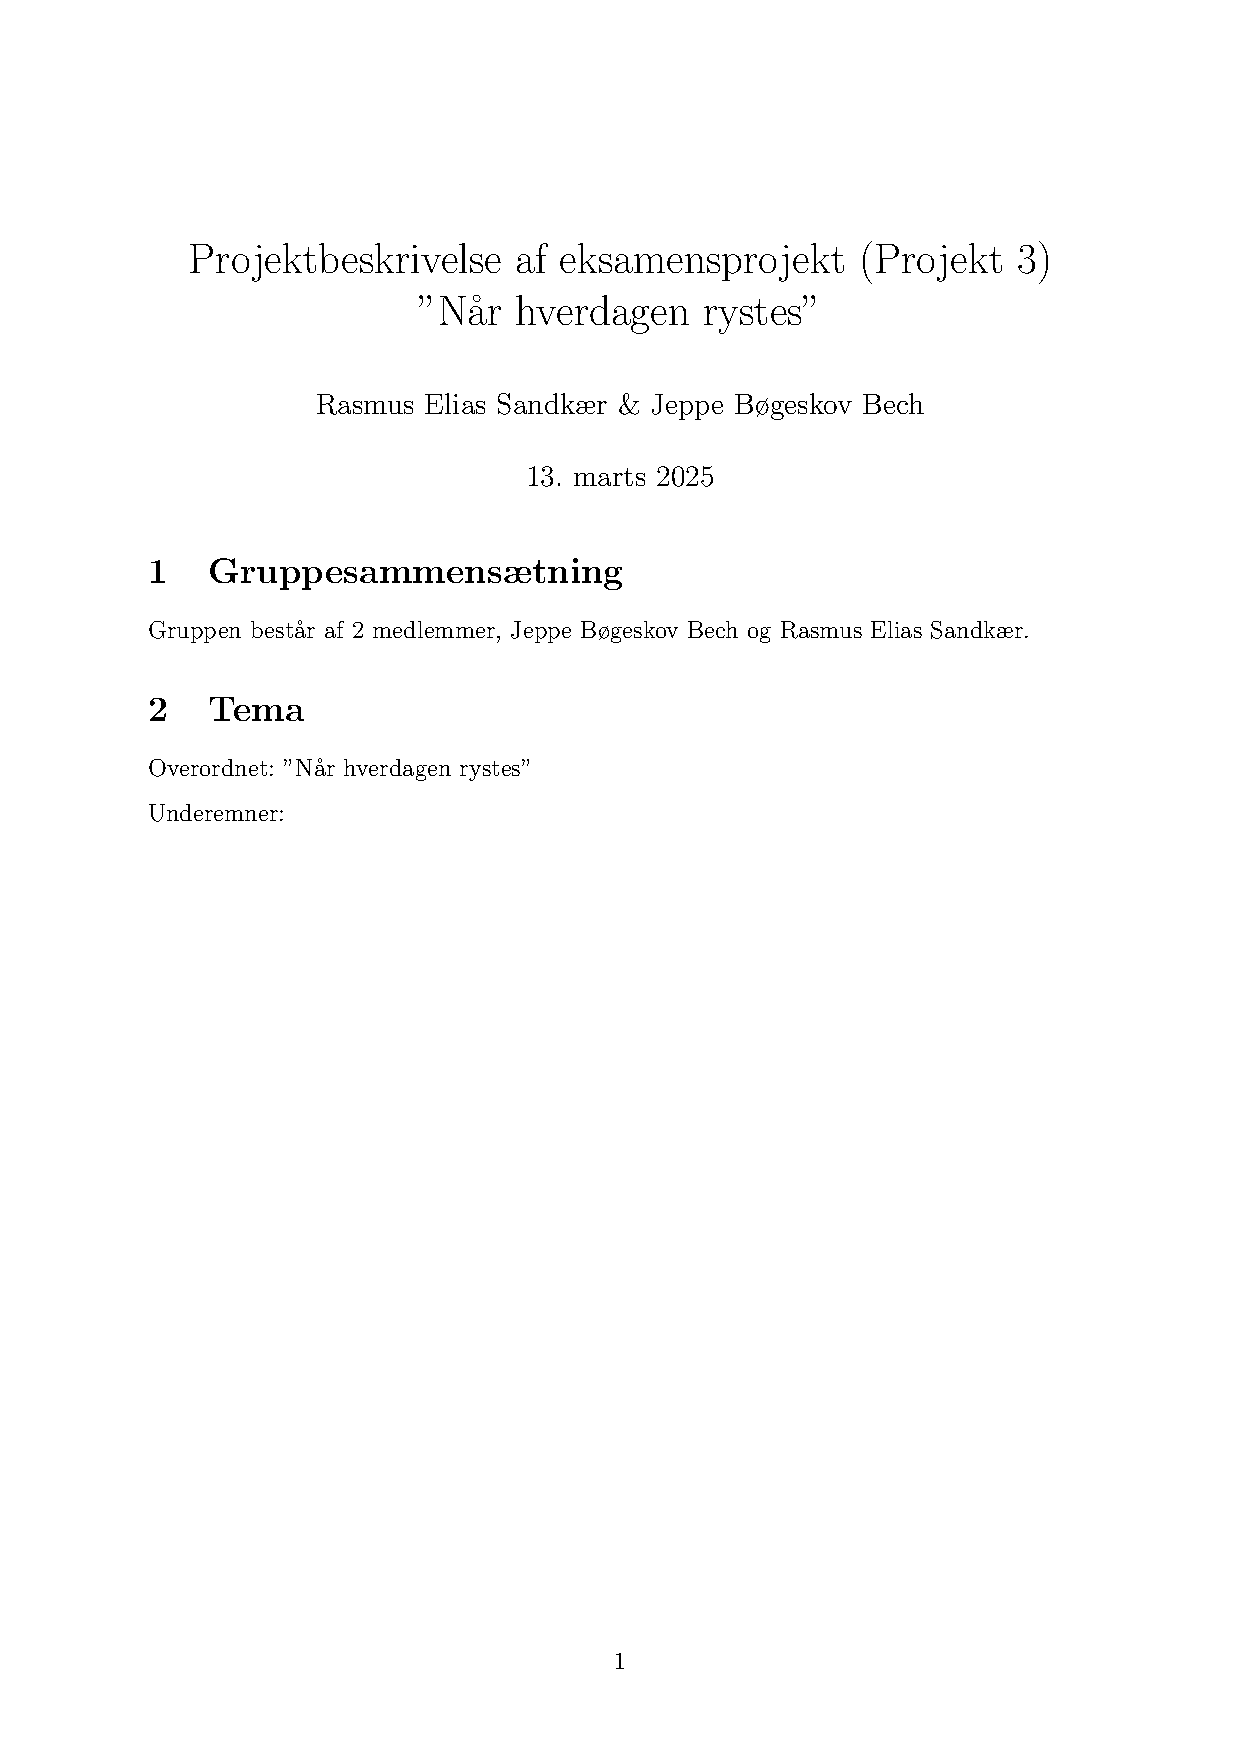
\includepdf[pages=-,delta=5 5,frame=true,landscape=false,nup=1x1,pagecommand={\thispagestyle{plain}}]{./projektbeskrivelse.pdf}
    \end{appendices}
\end{document}
